\section{Home} {
    Quando l'utente entra nella piattaforma si trova nella pagina iniziale ``\textbf{Home}''. \aCapo
    Se non ha deciso in precedenza la visione predefinita della guida, visualizzerà i luoghi sotto forma di una mappa. 
    Direttamente dalla pagina Home, si può cambiare la visualizzazione in mappa e viceversa (da mappa in lista), cliccando tale bottone:
    \begin{figure}[H]
        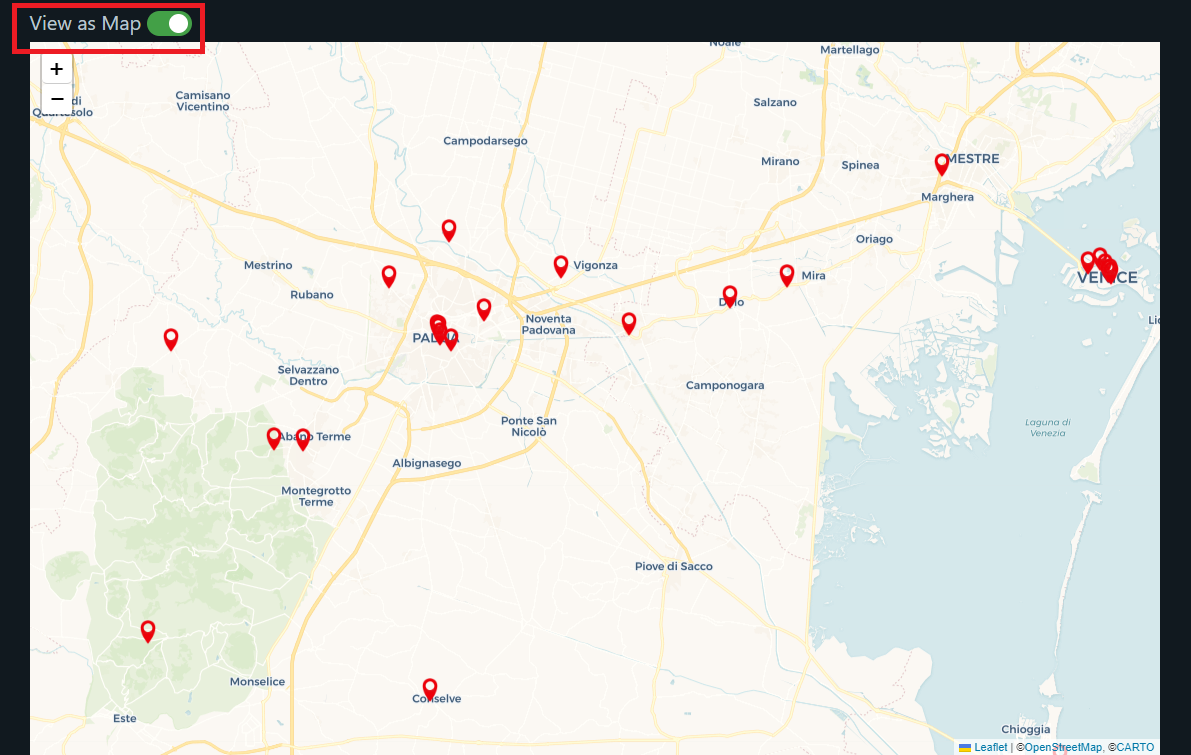
\includegraphics[width=12cm]{sezioni/images/home.png}
        \centering
        \caption{Visualizzazione predefinita della pagina Home}
    \end{figure}

    \subsection{Visualizzazione guida come lista} {
        L'utente vedrà un elenco di posti, generati dalle recensioni dei profili social seguiti dagli utenti della piattaforma \platform{}. \aCapo
        Ogni luogo è caratterizzato da tali informazioni: 
        \begin{itemize}
            \item Location: si tratta del nome del posto ed è un link, il quale una volta cliccato aprirà un popup con maggiori informazioni (§8.3); 
            \item Score: si tratta del punteggio che è attribuito al posto, su una scala da 0 a 5 stelle.
        \end{itemize}       
        \begin{figure}[H]
            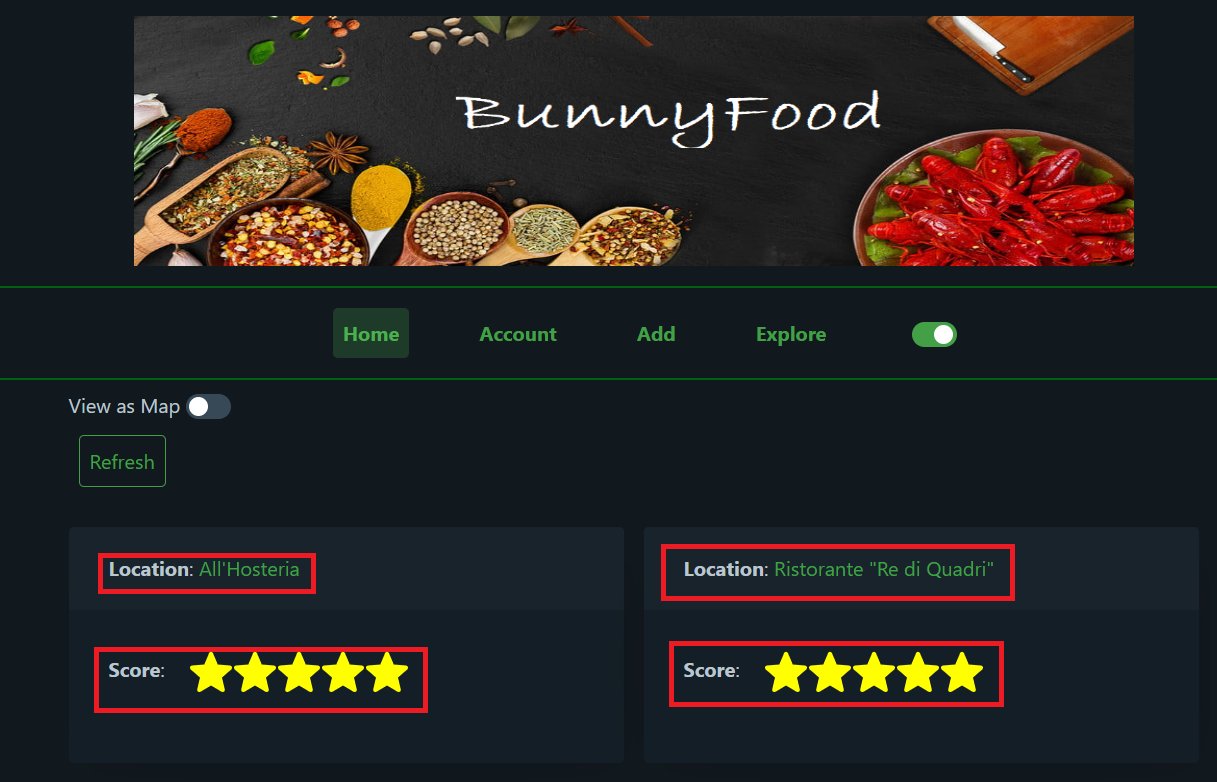
\includegraphics[width=12cm]{sezioni/images/list-home.png}
            \centering
            \caption{Visualizzazione lista locali nella pagina Home}
        \end{figure}
    }

    \subsection{Visualizzazione guida come mappa} {
        L'utente visulizzerà una mappa vera e propria con un ``segnaposto'' per la posizione di ogni posto. È possibile spostarsi sulla mappa, ingrandendo o diminuendo la visualizzazione. 
        Sono presenti infatti anche i tasti ``+'' e ``-'' per facilitare l'operazione di zoom. \aCapo
        Se il ``segnaposto'' viene cliccato compare il nome del luogo e il suo punteggio su una scala da 0 a 5. Il nome del posto, se cliccato, farà aprire un popup con maggiori informazioni (§8.3).

    }

    \subsection{Popup con maggiori informazioni} {
        Le informazioni che compaiono sono le seguenti:
        \begin{itemize}
            \item Il nome del posto;
            \item Una foto caratteristica di quel posto;
            \item Le categorie a cui appartiene il locale;
            \item L'indirizzo dove è situato il posto;
            \item Il numero telefonico del locale;
            \item Il suo punteggio su una scala da 0 a 5 stelle;
            \item Il link per il sito web di quel locale.
        \end{itemize}

        Per chiudere la finestra è necessario cliccare il tasto ``\textbf{Close}'' situato in alto a sinistra.
        \begin{figure}[H]
            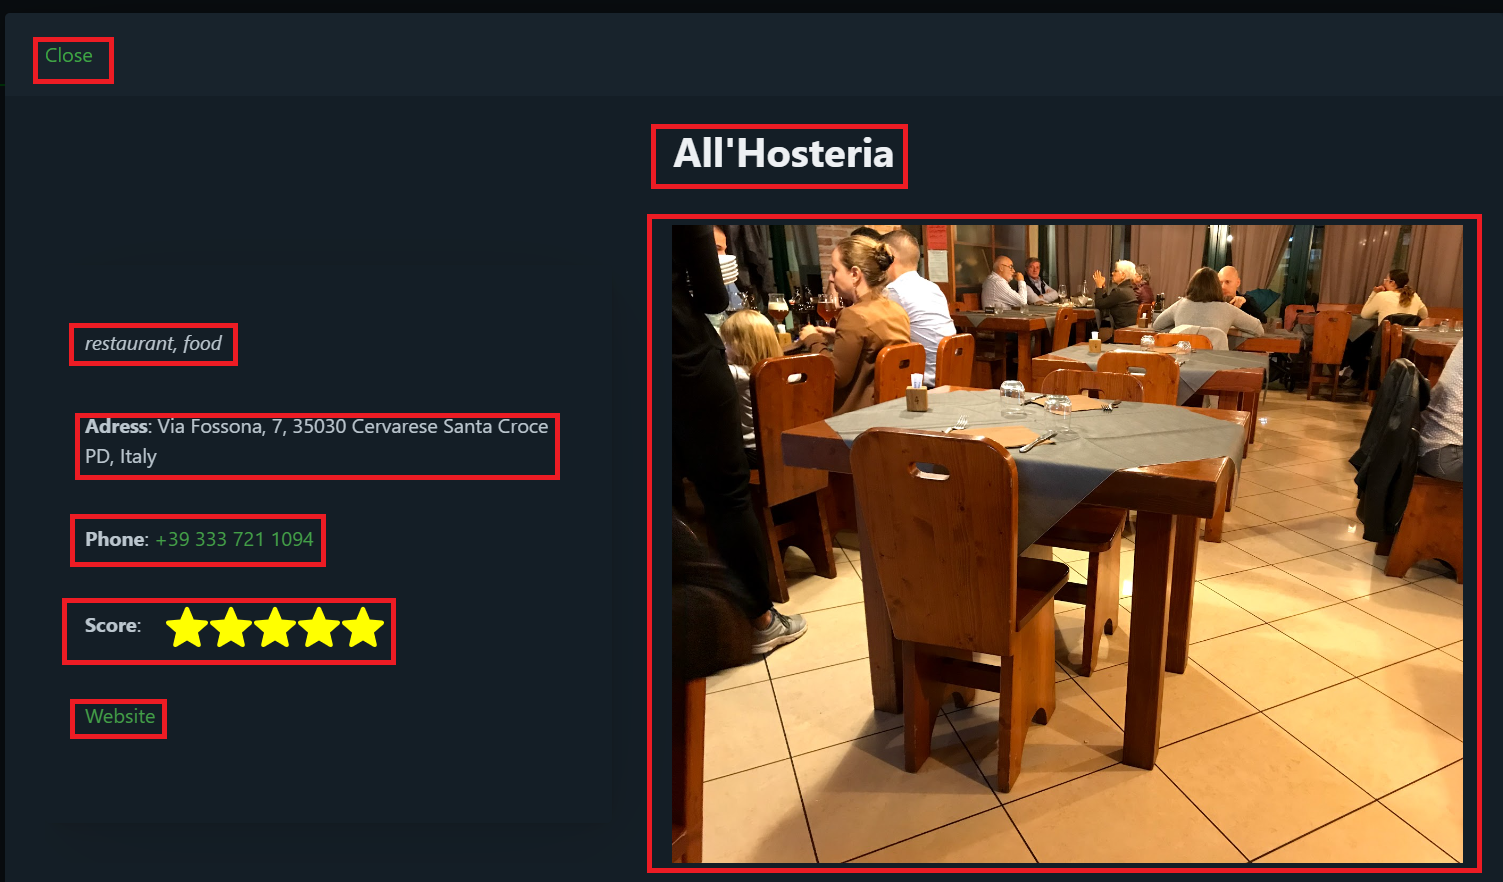
\includegraphics[width=12cm]{sezioni/images/popup.png}
            \centering
            \caption{Visualizzazione maggiori informazioni di un locale}
        \end{figure}
        }
}
